\documentclass[usenames,dvipsnames]{beamer}
\usepackage{eulervm}
\usepackage{mystyle1}
\title[Entanglement using Knots]{\huge Entanglement Classification using Knots \\{\large PH3203 Term Project}}
\author[Seth, Das, Karmakar]{{ Sagnik Seth} {\tiny{22MS026}} \and { Jessica  Das}  {\tiny{22MS157}} \and { Sayan Karmakar}  {\tiny{22MS163}}}
\institute[]{Instructor: Prof. Sourin Das\\[0.2cm]
	\textit{Department of Physics, IISER Kolkata}}
\date{}
\usetheme{Madrid}
\definecolor{bubbles}{rgb}{0.91, 1.0, 1.0}
\usecolortheme{whale}
\setbeamercolor{normal text}{fg=black,bg=bubbles!70}
\setbeamercolor{structure}{fg=red, bg=violet}

\setbeamercolor{alerted text}{fg=red!85!black}

\setbeamercolor{item projected}{use=item,fg=black,bg=item.fg!35}
\beamertemplatenavigationsymbolsempty
\setbeamercolor*{palette primary}{use=structure,fg=structure.fg}
\setbeamercolor*{palette secondary}{use=structure,fg=structure.fg!95!black}
\setbeamercolor*{palette tertiary}{use=structure,fg=structure.fg!90!black}
\setbeamercolor*{palette quaternary}{use=structure,fg=structure.fg!95!black,bg=black!80}

\setbeamercolor*{framesubtitle}{fg=white}

\setbeamercolor*{block title}{parent=structure,bg=black!60}
\setbeamercolor*{block body}{fg=black,bg=black!10}
\setbeamercolor*{block title alerted}{parent=alerted text,bg=black!15}
\setbeamercolor*{block title example}{parent=example text,bg=black!15}





% \setbeamertemplate{footline}{
%     \hfill
%     \scriptsize{
%         \insertshortauthor \quad (\insertshorttitle) \quad \insertshortdate
%         \hspace{1cm}
%         \insertframenumber\,/\,\inserttotalframenumber
%     }
%     \hspace{0.5cm}
%     \vspace{0.2cm}

\begin{document}
	
	\frame{\titlepage}
	
	
	\begin{frame}
		\begin{center}
			\textbf{\huge Basic Theoretical Background}
		\end{center}
	\end{frame}
	\begin{frame}{\textbf{\large Introduction to Knots}}
		
	\end{frame}
	\begin{frame}{\textbf{\large Introduction to Quantum Information}}
		
	\end{frame}
	\begin{frame}
		\begin{center}
			\textbf{\huge Classifying Entanglement using Knots}
		\end{center}
	\end{frame}
	\begin{frame}{\textbf{\large Polynomial Approach to Entangledment}}
		
	\end{frame}
	\begin{frame}{\textbf{Obtaining a Link from given State}}
		
	\end{frame}
	\begin{frame}{\textbf{Obtaining State from a given Link}}
		
	\end{frame}
	\begin{frame}
		\begin{center}
			\textbf{\Huge Some Examples...}
		\end{center}
	\end{frame}
	\begin{frame}{\textbf{Three Qubit System}: 3\textsuperscript{1} class}
		\textcolor{red}{\textbf{Pure State:} } $\ket{3^1}_{abc} = \frac{1}{\sqrt{2}}\brac{\ket{000}_{abc}+\ket{111}_{abc}}$\\[0.3cm]
		\begin{minipage}{0.35\textwidth}
			%

\tikzset{every picture/.style={line width=0.75pt}} %set default line width to 0.75pt        

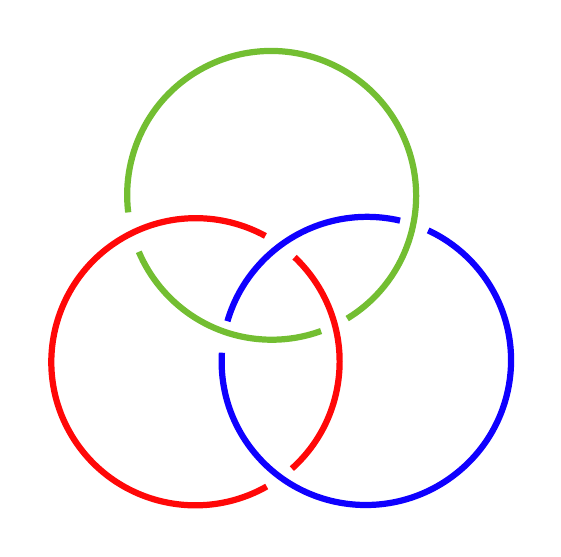
\begin{tikzpicture}[x=0.75pt,y=0.75pt,yscale=-1,xscale=1]
%uncomment if require: \path (0,300); %set diagram left start at 0, and has height of 300

%Shape: Arc [id:dp49278097545949884] 
\draw  [draw opacity=0][line width=2.25]  (328.62,163.73) .. controls (321.19,166.44) and (313.18,167.92) .. (304.82,167.92) .. controls (276.06,167.92) and (251.39,150.46) .. (240.8,125.56) -- (304.82,98.33) -- cycle ; \draw  [color={rgb, 255:red, 115; green, 190; blue, 50 }  ,draw opacity=1 ][line width=2.25]  (328.62,163.73) .. controls (321.19,166.44) and (313.18,167.92) .. (304.82,167.92) .. controls (276.06,167.92) and (251.39,150.46) .. (240.8,125.56) ;  
%Shape: Arc [id:dp7313937278600963] 
\draw  [draw opacity=0][line width=2.25]  (380.22,115.26) .. controls (389.75,119.69) and (398.4,126.36) .. (405.34,135.15) .. controls (429.07,165.23) and (423.73,208.87) .. (393.41,232.62) .. controls (363.09,256.37) and (319.27,251.24) .. (295.54,221.15) .. controls (284.6,207.29) and (279.84,190.54) .. (280.85,174.18) -- (350.44,178.15) -- cycle ; \draw  [color={rgb, 255:red, 15; green, 0; blue, 255 }  ,draw opacity=1 ][line width=2.25]  (380.22,115.26) .. controls (389.75,119.69) and (398.4,126.36) .. (405.34,135.15) .. controls (429.07,165.23) and (423.73,208.87) .. (393.41,232.62) .. controls (363.09,256.37) and (319.27,251.24) .. (295.54,221.15) .. controls (284.6,207.29) and (279.84,190.54) .. (280.85,174.18) ;  
%Shape: Arc [id:dp9082888658781946] 
\draw  [draw opacity=0][line width=2.25]  (235.71,106.58) .. controls (232.15,77.58) and (247.26,48.37) .. (275.16,35.34) .. controls (309.93,19.08) and (351.4,34.11) .. (367.78,68.91) .. controls (383.06,101.37) and (371.11,139.56) .. (341.2,157.73) -- (304.82,98.33) -- cycle ; \draw  [color={rgb, 255:red, 115; green, 190; blue, 50 }  ,draw opacity=1 ][line width=2.25]  (235.71,106.58) .. controls (232.15,77.58) and (247.26,48.37) .. (275.16,35.34) .. controls (309.93,19.08) and (351.4,34.11) .. (367.78,68.91) .. controls (383.06,101.37) and (371.11,139.56) .. (341.2,157.73) ;  
%Shape: Arc [id:dp7357603003827937] 
\draw  [draw opacity=0][line width=2.25]  (302.44,238.64) .. controls (269.08,257.52) and (226.71,245.99) .. (207.75,212.86) .. controls (188.77,179.69) and (200.44,137.44) .. (233.81,118.48) .. controls (255.62,106.09) and (281.32,106.72) .. (301.8,117.92) -- (268.17,178.53) -- cycle ; \draw  [color={rgb, 255:red, 255; green, 8; blue, 8 }  ,draw opacity=1 ][line width=2.25]  (302.44,238.64) .. controls (269.08,257.52) and (226.71,245.99) .. (207.75,212.86) .. controls (188.77,179.69) and (200.44,137.44) .. (233.81,118.48) .. controls (255.62,106.09) and (281.32,106.72) .. (301.8,117.92) ;  
%Shape: Arc [id:dp02993817280793909] 
\draw  [draw opacity=0][line width=2.25]  (283.51,159.01) .. controls (286.66,148.19) and (292.5,137.97) .. (301.03,129.39) .. controls (318.8,111.52) and (343.85,105.22) .. (366.69,110.55) -- (350.44,178.15) -- cycle ; \draw  [color={rgb, 255:red, 15; green, 0; blue, 255 }  ,draw opacity=1 ][line width=2.25]  (283.51,159.01) .. controls (286.66,148.19) and (292.5,137.97) .. (301.03,129.39) .. controls (318.8,111.52) and (343.85,105.22) .. (366.69,110.55) ;  
%Shape: Arc [id:dp6464277844327507] 
\draw  [draw opacity=0][line width=2.25]  (315.85,128.16) .. controls (331.94,143.37) and (340.46,165.99) .. (336.68,189.48) .. controls (334.06,205.76) and (325.96,219.8) .. (314.56,230.03) -- (268.17,178.53) -- cycle ; \draw  [color={rgb, 255:red, 255; green, 8; blue, 8 }  ,draw opacity=1 ][line width=2.25]  (315.85,128.16) .. controls (331.94,143.37) and (340.46,165.99) .. (336.68,189.48) .. controls (334.06,205.76) and (325.96,219.8) .. (314.56,230.03) ;  




\end{tikzpicture}
  % Make sure this file exists
			\scalebox{0.6}{

\tikzset{every picture/.style={line width=0.75pt}} %set default line width to 0.75pt        

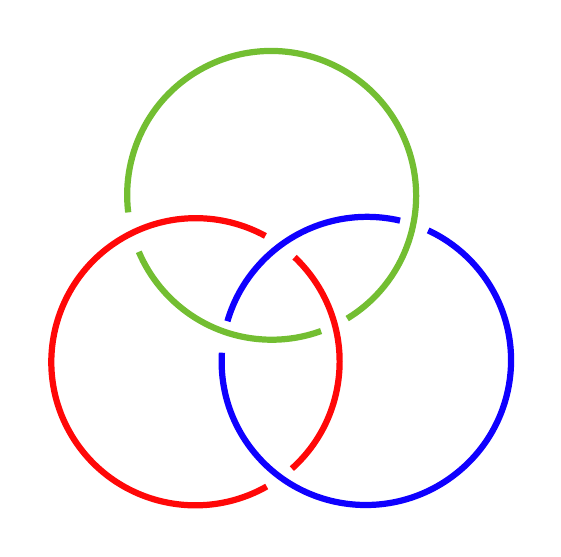
\begin{tikzpicture}[x=0.75pt,y=0.75pt,yscale=-1,xscale=1]
%uncomment if require: \path (0,300); %set diagram left start at 0, and has height of 300

%Shape: Arc [id:dp49278097545949884] 
\draw  [draw opacity=0][line width=2.25]  (328.62,163.73) .. controls (321.19,166.44) and (313.18,167.92) .. (304.82,167.92) .. controls (276.06,167.92) and (251.39,150.46) .. (240.8,125.56) -- (304.82,98.33) -- cycle ; \draw  [color={rgb, 255:red, 115; green, 190; blue, 50 }  ,draw opacity=1 ][line width=2.25]  (328.62,163.73) .. controls (321.19,166.44) and (313.18,167.92) .. (304.82,167.92) .. controls (276.06,167.92) and (251.39,150.46) .. (240.8,125.56) ;  
%Shape: Arc [id:dp7313937278600963] 
\draw  [draw opacity=0][line width=2.25]  (380.22,115.26) .. controls (389.75,119.69) and (398.4,126.36) .. (405.34,135.15) .. controls (429.07,165.23) and (423.73,208.87) .. (393.41,232.62) .. controls (363.09,256.37) and (319.27,251.24) .. (295.54,221.15) .. controls (284.6,207.29) and (279.84,190.54) .. (280.85,174.18) -- (350.44,178.15) -- cycle ; \draw  [color={rgb, 255:red, 15; green, 0; blue, 255 }  ,draw opacity=1 ][line width=2.25]  (380.22,115.26) .. controls (389.75,119.69) and (398.4,126.36) .. (405.34,135.15) .. controls (429.07,165.23) and (423.73,208.87) .. (393.41,232.62) .. controls (363.09,256.37) and (319.27,251.24) .. (295.54,221.15) .. controls (284.6,207.29) and (279.84,190.54) .. (280.85,174.18) ;  
%Shape: Arc [id:dp9082888658781946] 
\draw  [draw opacity=0][line width=2.25]  (235.71,106.58) .. controls (232.15,77.58) and (247.26,48.37) .. (275.16,35.34) .. controls (309.93,19.08) and (351.4,34.11) .. (367.78,68.91) .. controls (383.06,101.37) and (371.11,139.56) .. (341.2,157.73) -- (304.82,98.33) -- cycle ; \draw  [color={rgb, 255:red, 115; green, 190; blue, 50 }  ,draw opacity=1 ][line width=2.25]  (235.71,106.58) .. controls (232.15,77.58) and (247.26,48.37) .. (275.16,35.34) .. controls (309.93,19.08) and (351.4,34.11) .. (367.78,68.91) .. controls (383.06,101.37) and (371.11,139.56) .. (341.2,157.73) ;  
%Shape: Arc [id:dp7357603003827937] 
\draw  [draw opacity=0][line width=2.25]  (302.44,238.64) .. controls (269.08,257.52) and (226.71,245.99) .. (207.75,212.86) .. controls (188.77,179.69) and (200.44,137.44) .. (233.81,118.48) .. controls (255.62,106.09) and (281.32,106.72) .. (301.8,117.92) -- (268.17,178.53) -- cycle ; \draw  [color={rgb, 255:red, 255; green, 8; blue, 8 }  ,draw opacity=1 ][line width=2.25]  (302.44,238.64) .. controls (269.08,257.52) and (226.71,245.99) .. (207.75,212.86) .. controls (188.77,179.69) and (200.44,137.44) .. (233.81,118.48) .. controls (255.62,106.09) and (281.32,106.72) .. (301.8,117.92) ;  
%Shape: Arc [id:dp02993817280793909] 
\draw  [draw opacity=0][line width=2.25]  (283.51,159.01) .. controls (286.66,148.19) and (292.5,137.97) .. (301.03,129.39) .. controls (318.8,111.52) and (343.85,105.22) .. (366.69,110.55) -- (350.44,178.15) -- cycle ; \draw  [color={rgb, 255:red, 15; green, 0; blue, 255 }  ,draw opacity=1 ][line width=2.25]  (283.51,159.01) .. controls (286.66,148.19) and (292.5,137.97) .. (301.03,129.39) .. controls (318.8,111.52) and (343.85,105.22) .. (366.69,110.55) ;  
%Shape: Arc [id:dp6464277844327507] 
\draw  [draw opacity=0][line width=2.25]  (315.85,128.16) .. controls (331.94,143.37) and (340.46,165.99) .. (336.68,189.48) .. controls (334.06,205.76) and (325.96,219.8) .. (314.56,230.03) -- (268.17,178.53) -- cycle ; \draw  [color={rgb, 255:red, 255; green, 8; blue, 8 }  ,draw opacity=1 ][line width=2.25]  (315.85,128.16) .. controls (331.94,143.37) and (340.46,165.99) .. (336.68,189.48) .. controls (334.06,205.76) and (325.96,219.8) .. (314.56,230.03) ;  




\end{tikzpicture}
}
			\begin{itemize}
				\item \textbf{Eigenvalues:} $0.0,\ 0.5,\ \mathcolor{red}{-0.5}$
				\item One eigenvalue is negative $\rightarrow$ \textbf{\textcolor{OliveGreen}{Tripartite Entanglement}}
			\end{itemize}
		\end{minipage}%
		\begin{minipage}{0.5\textwidth}
			\footnotesize
			\begin{equation*}
				\rho_{abc} =
				\left[
				\begin{array}{cccccccc}
				0.5 & 0.0 & 0.0 & 0.0 & 0.0 & 0.0 & 0.0 & 0.5 \\
				0.0 & 0.0 & 0.0 & 0.0 & 0.0 & 0.0 & 0.0 & 0.0 \\
				0.0 & 0.0 & 0.0 & 0.0 & 0.0 & 0.0 & 0.0 & 0.0 \\
				0.0 & 0.0 & 0.0 & 0.0 & 0.0 & 0.0 & 0.0 & 0.0 \\
				0.0 & 0.0 & 0.0 & 0.0 & 0.0 & 0.0 & 0.0 & 0.0 \\
				0.0 & 0.0 & 0.0 & 0.0 & 0.0 & 0.0 & 0.0 & 0.0 \\
				0.0 & 0.0 & 0.0 & 0.0 & 0.0 & 0.0 & 0.0 & 0.0 \\
				0.5 & 0.0 & 0.0 & 0.0 & 0.0 & 0.0 & 0.0 & 0.5 \\
				\end{array}
				\right]
			\end{equation*}
			\begin{equation*}
				\rho^{T_a}_{abc} =
				\left[
				\begin{array}{cccccccc}
				0.5 & 0.0 & 0.0 & 0.0 & 0.0 & 0.0 & 0.0 & 0.0 \\
				0.0 & 0.0 & 0.0 & 0.0 & 0.0 & 0.0 & 0.0 & 0.0 \\
				0.0 & 0.0 & 0.0 & 0.0 & 0.0 & 0.0 & 0.0 & 0.0 \\
				0.0 & 0.0 & 0.0 & 0.0 & 0.5 & 0.0 & 0.0 & 0.0 \\
				0.0 & 0.0 & 0.0 & 0.5 & 0.0 & 0.0 & 0.0 & 0.0 \\
				0.0 & 0.0 & 0.0 & 0.0 & 0.0 & 0.0 & 0.0 & 0.0 \\
				0.0 & 0.0 & 0.0 & 0.0 & 0.0 & 0.0 & 0.0 & 0.0 \\
				0.0 & 0.0 & 0.0 & 0.0 & 0.0 & 0.0 & 0.0 & 0.5 \\
				\end{array}
				\right]
				\end{equation*}
		\end{minipage}
	\end{frame}
	\begin{frame}{\textbf{Three Qubit System}: 3\textsuperscript{1} class}
		\textcolor{red}{\textbf{Pure State:} } $\ket{3^1}_{abc} = \frac{1}{\sqrt{2}}\brac{\ket{000}_{abc}+\ket{111}_{abc}}$\\[0.3cm]
		\begin{minipage}{0.35\textwidth}
			%

\tikzset{every picture/.style={line width=0.75pt}} %set default line width to 0.75pt        

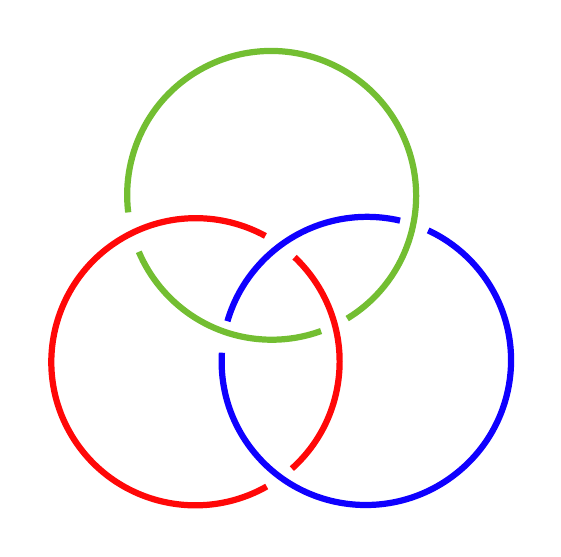
\begin{tikzpicture}[x=0.75pt,y=0.75pt,yscale=-1,xscale=1]
%uncomment if require: \path (0,300); %set diagram left start at 0, and has height of 300

%Shape: Arc [id:dp49278097545949884] 
\draw  [draw opacity=0][line width=2.25]  (328.62,163.73) .. controls (321.19,166.44) and (313.18,167.92) .. (304.82,167.92) .. controls (276.06,167.92) and (251.39,150.46) .. (240.8,125.56) -- (304.82,98.33) -- cycle ; \draw  [color={rgb, 255:red, 115; green, 190; blue, 50 }  ,draw opacity=1 ][line width=2.25]  (328.62,163.73) .. controls (321.19,166.44) and (313.18,167.92) .. (304.82,167.92) .. controls (276.06,167.92) and (251.39,150.46) .. (240.8,125.56) ;  
%Shape: Arc [id:dp7313937278600963] 
\draw  [draw opacity=0][line width=2.25]  (380.22,115.26) .. controls (389.75,119.69) and (398.4,126.36) .. (405.34,135.15) .. controls (429.07,165.23) and (423.73,208.87) .. (393.41,232.62) .. controls (363.09,256.37) and (319.27,251.24) .. (295.54,221.15) .. controls (284.6,207.29) and (279.84,190.54) .. (280.85,174.18) -- (350.44,178.15) -- cycle ; \draw  [color={rgb, 255:red, 15; green, 0; blue, 255 }  ,draw opacity=1 ][line width=2.25]  (380.22,115.26) .. controls (389.75,119.69) and (398.4,126.36) .. (405.34,135.15) .. controls (429.07,165.23) and (423.73,208.87) .. (393.41,232.62) .. controls (363.09,256.37) and (319.27,251.24) .. (295.54,221.15) .. controls (284.6,207.29) and (279.84,190.54) .. (280.85,174.18) ;  
%Shape: Arc [id:dp9082888658781946] 
\draw  [draw opacity=0][line width=2.25]  (235.71,106.58) .. controls (232.15,77.58) and (247.26,48.37) .. (275.16,35.34) .. controls (309.93,19.08) and (351.4,34.11) .. (367.78,68.91) .. controls (383.06,101.37) and (371.11,139.56) .. (341.2,157.73) -- (304.82,98.33) -- cycle ; \draw  [color={rgb, 255:red, 115; green, 190; blue, 50 }  ,draw opacity=1 ][line width=2.25]  (235.71,106.58) .. controls (232.15,77.58) and (247.26,48.37) .. (275.16,35.34) .. controls (309.93,19.08) and (351.4,34.11) .. (367.78,68.91) .. controls (383.06,101.37) and (371.11,139.56) .. (341.2,157.73) ;  
%Shape: Arc [id:dp7357603003827937] 
\draw  [draw opacity=0][line width=2.25]  (302.44,238.64) .. controls (269.08,257.52) and (226.71,245.99) .. (207.75,212.86) .. controls (188.77,179.69) and (200.44,137.44) .. (233.81,118.48) .. controls (255.62,106.09) and (281.32,106.72) .. (301.8,117.92) -- (268.17,178.53) -- cycle ; \draw  [color={rgb, 255:red, 255; green, 8; blue, 8 }  ,draw opacity=1 ][line width=2.25]  (302.44,238.64) .. controls (269.08,257.52) and (226.71,245.99) .. (207.75,212.86) .. controls (188.77,179.69) and (200.44,137.44) .. (233.81,118.48) .. controls (255.62,106.09) and (281.32,106.72) .. (301.8,117.92) ;  
%Shape: Arc [id:dp02993817280793909] 
\draw  [draw opacity=0][line width=2.25]  (283.51,159.01) .. controls (286.66,148.19) and (292.5,137.97) .. (301.03,129.39) .. controls (318.8,111.52) and (343.85,105.22) .. (366.69,110.55) -- (350.44,178.15) -- cycle ; \draw  [color={rgb, 255:red, 15; green, 0; blue, 255 }  ,draw opacity=1 ][line width=2.25]  (283.51,159.01) .. controls (286.66,148.19) and (292.5,137.97) .. (301.03,129.39) .. controls (318.8,111.52) and (343.85,105.22) .. (366.69,110.55) ;  
%Shape: Arc [id:dp6464277844327507] 
\draw  [draw opacity=0][line width=2.25]  (315.85,128.16) .. controls (331.94,143.37) and (340.46,165.99) .. (336.68,189.48) .. controls (334.06,205.76) and (325.96,219.8) .. (314.56,230.03) -- (268.17,178.53) -- cycle ; \draw  [color={rgb, 255:red, 255; green, 8; blue, 8 }  ,draw opacity=1 ][line width=2.25]  (315.85,128.16) .. controls (331.94,143.37) and (340.46,165.99) .. (336.68,189.48) .. controls (334.06,205.76) and (325.96,219.8) .. (314.56,230.03) ;  




\end{tikzpicture}
  % Make sure this file exists
			\scalebox{0.6}{

\tikzset{every picture/.style={line width=0.75pt}} %set default line width to 0.75pt        

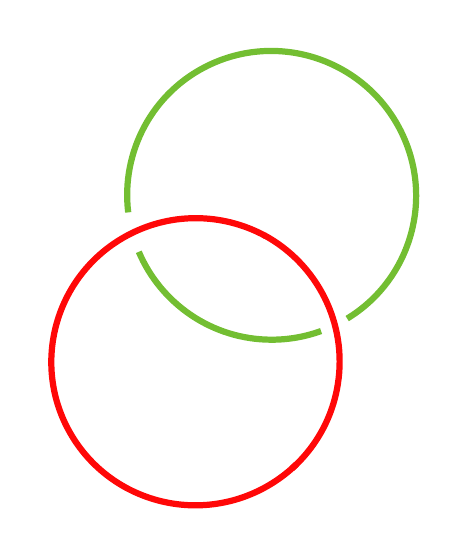
\begin{tikzpicture}[x=0.75pt,y=0.75pt,yscale=-1,xscale=1]
%uncomment if require: \path (0,300); %set diagram left start at 0, and has height of 300

%Shape: Arc [id:dp9961343423853242] 
\draw  [draw opacity=0][line width=2.25]  (348.62,177.2) .. controls (341.19,179.91) and (333.18,181.38) .. (324.82,181.38) .. controls (296.06,181.38) and (271.39,163.93) .. (260.8,139.03) -- (324.82,111.8) -- cycle ; \draw  [color={rgb, 255:red, 115; green, 190; blue, 50 }  ,draw opacity=1 ][line width=2.25]  (348.62,177.2) .. controls (341.19,179.91) and (333.18,181.38) .. (324.82,181.38) .. controls (296.06,181.38) and (271.39,163.93) .. (260.8,139.03) ;  
%Shape: Arc [id:dp11612154435512079] 
\draw  [draw opacity=0][line width=2.25]  (255.71,120.05) .. controls (252.15,91.05) and (267.26,61.84) .. (295.16,48.8) .. controls (329.93,32.55) and (371.4,47.58) .. (387.78,82.37) .. controls (403.06,114.84) and (391.11,153.03) .. (361.2,171.2) -- (324.82,111.8) -- cycle ; \draw  [color={rgb, 255:red, 115; green, 190; blue, 50 }  ,draw opacity=1 ][line width=2.25]  (255.71,120.05) .. controls (252.15,91.05) and (267.26,61.84) .. (295.16,48.8) .. controls (329.93,32.55) and (371.4,47.58) .. (387.78,82.37) .. controls (403.06,114.84) and (391.11,153.03) .. (361.2,171.2) ;  
%Shape: Arc [id:dp5786194174920847] 
\draw  [draw opacity=0][line width=2.25]  (336.8,241.34) .. controls (332.62,245.42) and (327.85,249.03) .. (322.53,252.05) .. controls (289.16,271.01) and (246.73,259.49) .. (227.75,226.32) .. controls (208.77,193.16) and (220.44,150.91) .. (253.81,131.95) .. controls (275.62,119.56) and (301.32,120.19) .. (321.8,131.39) -- (288.17,192) -- cycle ; \draw  [color={rgb, 255:red, 255; green, 8; blue, 8 }  ,draw opacity=1 ][line width=2.25]  (336.8,241.34) .. controls (332.62,245.42) and (327.85,249.03) .. (322.53,252.05) .. controls (289.16,271.01) and (246.73,259.49) .. (227.75,226.32) .. controls (208.77,193.16) and (220.44,150.91) .. (253.81,131.95) .. controls (275.62,119.56) and (301.32,120.19) .. (321.8,131.39) ;  
%Shape: Arc [id:dp2668566217368272] 
\draw  [draw opacity=0][line width=2.25]  (321.26,131.06) .. controls (346.43,144.68) and (361.48,173.11) .. (356.68,202.95) .. controls (354.06,219.23) and (345.96,233.27) .. (334.56,243.5) -- (288.17,192) -- cycle ; \draw  [color={rgb, 255:red, 255; green, 8; blue, 8 }  ,draw opacity=1 ][line width=2.25]  (321.26,131.06) .. controls (346.43,144.68) and (361.48,173.11) .. (356.68,202.95) .. controls (354.06,219.23) and (345.96,233.27) .. (334.56,243.5) ;  




\end{tikzpicture}
}
			\begin{itemize}
				\item \textbf{Eigenvalues:} $0.0,\ 0.5\geq0$
			\end{itemize}
		\end{minipage}%
		\begin{minipage}{0.5\textwidth}
			\footnotesize
			\begin{equation*}
				\rho_{ab}
				\left[
				\begin{array}{cccc}
				0.5 & 0.0 & 0.0 & 0.0 \\
				0.0 & 0.0 & 0.0 & 0.0 \\
				0.0 & 0.0 & 0.0 & 0.0 \\
				0.0 & 0.0 & 0.0 & 0.5 \\
				\end{array}
				\right]
				\end{equation*} 
				\begin{equation*}
					\rho^{Ta}_{ab}
					\left[
					\begin{array}{cccc}
					0.5 & 0.0 & 0.0 & 0.0 \\
					0.0 & 0.0 & 0.0 & 0.0 \\
					0.0 & 0.0 & 0.0 & 0.0 \\
					0.0 & 0.0 & 0.0 & 0.5 \\
					\end{array}
					\right]
					\end{equation*}
				\begin{itemize}
					\item All eigenvalues are positive.
					\item System completely \textbf{separable} after cut.
				\end{itemize}
		\end{minipage}
	\end{frame}





	\begin{frame}{\textbf{Three Qubit System}: 3\textsuperscript{2} class}
		\textcolor{red}{\textbf{Pure State:} } $\ket{3^2}_{abc} = \frac{1}{\sqrt{3}}\brac{\ket{000}_{abc} + \ket{111}_{abc} + \ket{001}_{abc}} $\\[0.3cm]
		\begin{minipage}{0.35\textwidth}
			%

\tikzset{every picture/.style={line width=0.75pt}} %set default line width to 0.75pt        

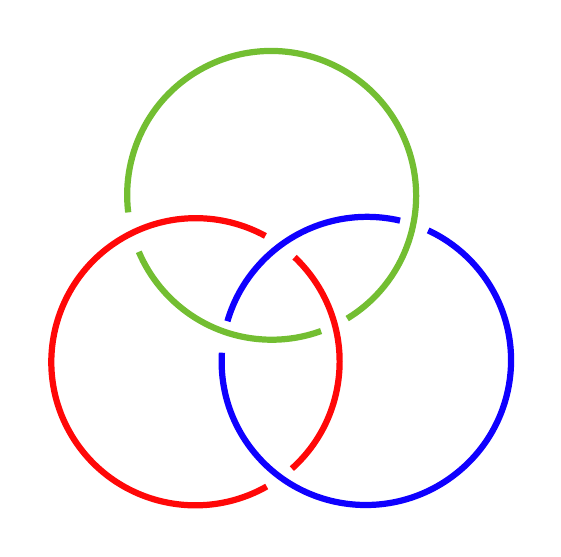
\begin{tikzpicture}[x=0.75pt,y=0.75pt,yscale=-1,xscale=1]
%uncomment if require: \path (0,300); %set diagram left start at 0, and has height of 300

%Shape: Arc [id:dp49278097545949884] 
\draw  [draw opacity=0][line width=2.25]  (328.62,163.73) .. controls (321.19,166.44) and (313.18,167.92) .. (304.82,167.92) .. controls (276.06,167.92) and (251.39,150.46) .. (240.8,125.56) -- (304.82,98.33) -- cycle ; \draw  [color={rgb, 255:red, 115; green, 190; blue, 50 }  ,draw opacity=1 ][line width=2.25]  (328.62,163.73) .. controls (321.19,166.44) and (313.18,167.92) .. (304.82,167.92) .. controls (276.06,167.92) and (251.39,150.46) .. (240.8,125.56) ;  
%Shape: Arc [id:dp7313937278600963] 
\draw  [draw opacity=0][line width=2.25]  (380.22,115.26) .. controls (389.75,119.69) and (398.4,126.36) .. (405.34,135.15) .. controls (429.07,165.23) and (423.73,208.87) .. (393.41,232.62) .. controls (363.09,256.37) and (319.27,251.24) .. (295.54,221.15) .. controls (284.6,207.29) and (279.84,190.54) .. (280.85,174.18) -- (350.44,178.15) -- cycle ; \draw  [color={rgb, 255:red, 15; green, 0; blue, 255 }  ,draw opacity=1 ][line width=2.25]  (380.22,115.26) .. controls (389.75,119.69) and (398.4,126.36) .. (405.34,135.15) .. controls (429.07,165.23) and (423.73,208.87) .. (393.41,232.62) .. controls (363.09,256.37) and (319.27,251.24) .. (295.54,221.15) .. controls (284.6,207.29) and (279.84,190.54) .. (280.85,174.18) ;  
%Shape: Arc [id:dp9082888658781946] 
\draw  [draw opacity=0][line width=2.25]  (235.71,106.58) .. controls (232.15,77.58) and (247.26,48.37) .. (275.16,35.34) .. controls (309.93,19.08) and (351.4,34.11) .. (367.78,68.91) .. controls (383.06,101.37) and (371.11,139.56) .. (341.2,157.73) -- (304.82,98.33) -- cycle ; \draw  [color={rgb, 255:red, 115; green, 190; blue, 50 }  ,draw opacity=1 ][line width=2.25]  (235.71,106.58) .. controls (232.15,77.58) and (247.26,48.37) .. (275.16,35.34) .. controls (309.93,19.08) and (351.4,34.11) .. (367.78,68.91) .. controls (383.06,101.37) and (371.11,139.56) .. (341.2,157.73) ;  
%Shape: Arc [id:dp7357603003827937] 
\draw  [draw opacity=0][line width=2.25]  (302.44,238.64) .. controls (269.08,257.52) and (226.71,245.99) .. (207.75,212.86) .. controls (188.77,179.69) and (200.44,137.44) .. (233.81,118.48) .. controls (255.62,106.09) and (281.32,106.72) .. (301.8,117.92) -- (268.17,178.53) -- cycle ; \draw  [color={rgb, 255:red, 255; green, 8; blue, 8 }  ,draw opacity=1 ][line width=2.25]  (302.44,238.64) .. controls (269.08,257.52) and (226.71,245.99) .. (207.75,212.86) .. controls (188.77,179.69) and (200.44,137.44) .. (233.81,118.48) .. controls (255.62,106.09) and (281.32,106.72) .. (301.8,117.92) ;  
%Shape: Arc [id:dp02993817280793909] 
\draw  [draw opacity=0][line width=2.25]  (283.51,159.01) .. controls (286.66,148.19) and (292.5,137.97) .. (301.03,129.39) .. controls (318.8,111.52) and (343.85,105.22) .. (366.69,110.55) -- (350.44,178.15) -- cycle ; \draw  [color={rgb, 255:red, 15; green, 0; blue, 255 }  ,draw opacity=1 ][line width=2.25]  (283.51,159.01) .. controls (286.66,148.19) and (292.5,137.97) .. (301.03,129.39) .. controls (318.8,111.52) and (343.85,105.22) .. (366.69,110.55) ;  
%Shape: Arc [id:dp6464277844327507] 
\draw  [draw opacity=0][line width=2.25]  (315.85,128.16) .. controls (331.94,143.37) and (340.46,165.99) .. (336.68,189.48) .. controls (334.06,205.76) and (325.96,219.8) .. (314.56,230.03) -- (268.17,178.53) -- cycle ; \draw  [color={rgb, 255:red, 255; green, 8; blue, 8 }  ,draw opacity=1 ][line width=2.25]  (315.85,128.16) .. controls (331.94,143.37) and (340.46,165.99) .. (336.68,189.48) .. controls (334.06,205.76) and (325.96,219.8) .. (314.56,230.03) ;  




\end{tikzpicture}
  % Make sure this file exists
			\begin{figure}
			\scalebox{0.4}{

\tikzset{every picture/.style={line width=0.75pt}} %set default line width to 0.75pt        

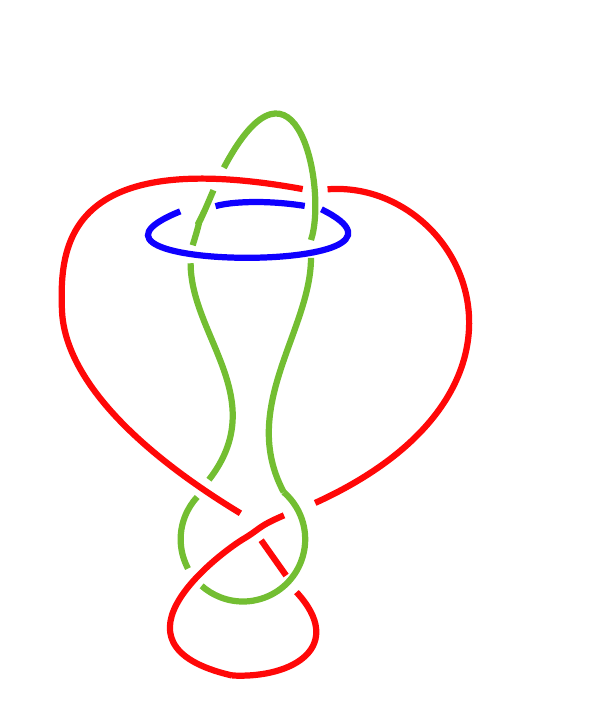
\begin{tikzpicture}[x=0.75pt,y=0.75pt,yscale=-1,xscale=1]
%uncomment if require: \path (0,300); %set diagram left start at 0, and has height of 300

%Curve Lines [id:da09943248726534226] 
\draw [color={rgb, 255:red, 255; green, 8; blue, 8 }  ,draw opacity=1 ][line width=2.25]    (343,46.68) .. controls (407,41.68) and (460,141.77) .. (337,197.77) ;
%Curve Lines [id:da6322873360352863] 
\draw [color={rgb, 255:red, 255; green, 8; blue, 8 }  ,draw opacity=1 ][line width=2.25]    (322,203.75) .. controls (309.03,209.29) and (311.19,209.93) .. (302.21,215.27) .. controls (293.23,220.61) and (231,265.75) .. (297,280.92) ;
%Curve Lines [id:da5011644671112231] 
\draw [color={rgb, 255:red, 255; green, 8; blue, 8 }  ,draw opacity=1 ][line width=2.25]    (331,46.57) .. controls (216,25.57) and (214,74.97) .. (215,104.68) .. controls (216,134.4) and (245,168.77) .. (301,202.77) ;
%Curve Lines [id:da44718777975671287] 
\draw [color={rgb, 255:red, 255; green, 8; blue, 8 }  ,draw opacity=1 ][line width=2.25]    (328,240.75) .. controls (352,266.75) and (326.73,282.41) .. (297,280.92) ;
%Shape: Arc [id:dp40054047053808206] 
\draw  [draw opacity=0][line width=2.25]  (321.85,192.58) .. controls (331.21,200.68) and (334.92,214.11) .. (330.11,226.28) .. controls (324.03,241.69) and (306.61,249.26) .. (291.19,243.17) .. controls (287.84,241.85) and (284.86,239.99) .. (282.31,237.73) -- (302.21,215.27) -- cycle ; \draw  [color={rgb, 255:red, 115; green, 190; blue, 50 }  ,draw opacity=1 ][line width=2.25]  (321.85,192.58) .. controls (331.21,200.68) and (334.92,214.11) .. (330.11,226.28) .. controls (324.03,241.69) and (306.61,249.26) .. (291.19,243.17) .. controls (287.84,241.85) and (284.86,239.99) .. (282.31,237.73) ;  
%Shape: Arc [id:dp11594177788693838] 
\draw  [draw opacity=0][line width=2.25]  (275.74,229.39) .. controls (271.75,221.9) and (270.94,212.77) .. (274.3,204.25) .. controls (275.71,200.7) and (277.71,197.56) .. (280.16,194.91) -- (302.21,215.27) -- cycle ; \draw  [color={rgb, 255:red, 115; green, 190; blue, 50 }  ,draw opacity=1 ][line width=2.25]  (275.74,229.39) .. controls (271.75,221.9) and (270.94,212.77) .. (274.3,204.25) .. controls (275.71,200.7) and (277.71,197.56) .. (280.16,194.91) ;  
%Straight Lines [id:da5976132825673692] 
\draw [color={rgb, 255:red, 255; green, 8; blue, 8 }  ,draw opacity=1 ][fill={rgb, 255:red, 208; green, 2; blue, 27 }  ,fill opacity=1 ][line width=2.25]    (311,215.75) -- (323,232.75) ;
%Curve Lines [id:da5325527173421334] 
\draw [color={rgb, 255:red, 115; green, 190; blue, 50 }  ,draw opacity=1 ][line width=2.25]    (335,79.68) .. controls (335,114.68) and (300,151.68) .. (321.85,192.58) ;
%Curve Lines [id:da2732197209903964] 
\draw [color={rgb, 255:red, 115; green, 190; blue, 50 }  ,draw opacity=1 ][line width=2.25]    (277,82.3) .. controls (277,117.3) and (316,147.68) .. (285.85,186.58) ;
%Curve Lines [id:da21608820690853647] 
\draw [color={rgb, 255:red, 115; green, 190; blue, 50 }  ,draw opacity=1 ][line width=2.25]    (278,73.65) .. controls (286,47.65) and (274,80.12) .. (288,47.12) ;
%Curve Lines [id:da1149451703987957] 
\draw [color={rgb, 255:red, 115; green, 190; blue, 50 }  ,draw opacity=1 ][line width=2.25]    (335,71.12) .. controls (343,47.12) and (328,-29.7) .. (293,36.3) ;
%Curve Lines [id:da6104443808138464] 
\draw [color={rgb, 255:red, 15; green, 0; blue, 255 }  ,draw opacity=1 ][line width=2.25]    (272,57.3) .. controls (200,86.3) and (405,88.3) .. (340,56.3) ;
%Curve Lines [id:da9503680162575591] 
\draw [color={rgb, 255:red, 15; green, 0; blue, 255 }  ,draw opacity=1 ][line width=2.25]    (289,54.8) .. controls (296,52.68) and (313,51.68) .. (332,54.68) ;




\end{tikzpicture}
}\end{figure}
			\begin{itemize}
				\item \textbf{Eigenvalues:} {\tiny $ \mathcolor{OliveGreen}{ \mathbf{-0.471}, 0.0, 0.333, 0.471, 0.666$}}\\{\tiny $ \mathcolor{red}{   \mathbf{-0.333}, 0.0, 0.127, 0.333, 0.872$}}
				\item \small One eigenvalue is negative $\rightarrow$ \textbf{\textcolor{OliveGreen}{Tripartite Entanglement}}
				 \end{itemize}
		\end{minipage}%
		\begin{minipage}{0.5\textwidth}
			\tiny  
			\begin{align*}
				\rho_{abc} &=
				\left[
				\begin{array}{cccccccc}
				0.333 & 0.333 & 0.0 & 0.0 & 0.0 & 0.0 & 0.0 & 0.333 \\ 
				0.333 & 0.333 & 0.0 & 0.0 & 0.0 & 0.0 & 0.0 & 0.333 \\ 
				0.0 & 0.0 & 0.0 & 0.0 & 0.0 & 0.0 & 0.0 & 0.0 \\ 
				0.0 & 0.0 & 0.0 & 0.0 & 0.0 & 0.0 & 0.0 & 0.0 \\ 
				0.0 & 0.0 & 0.0 & 0.0 & 0.0 & 0.0 & 0.0 & 0.0 \\ 
				0.0 & 0.0 & 0.0 & 0.0 & 0.0 & 0.0 & 0.0 & 0.0 \\ 
				0.0 & 0.0 & 0.0 & 0.0 & 0.0 & 0.0 & 0.0 & 0.0 \\ 
				0.333 & 0.333 & 0.0 & 0.0 & 0.0 & 0.0 & 0.0 & 0.333 \\ 
				\end{array}
				\right]
				\\
				\mathcolor{OliveGreen}{\rho^{T_a}_{abc}} &=
				\left[
				\begin{array}{cccccccc}
				0.333 & 0.333 & 0.0 & 0.0 & 0.0 & 0.0 & 0.0 & 0.0 \\ 
				0.333 & 0.333 & 0.0 & 0.0 & 0.0 & 0.0 & 0.0 & 0.0 \\ 
				0.0 & 0.0 & 0.0 & 0.0 & 0.0 & 0.0 & 0.0 & 0.0 \\ 
				0.0 & 0.0 & 0.0 & 0.0 & 0.333 & 0.333 & 0.0 & 0.0 \\ 
				0.0 & 0.0 & 0.0 & 0.333 & 0.0 & 0.0 & 0.0 & 0.0 \\ 
				0.0 & 0.0 & 0.0 & 0.333 & 0.0 & 0.0 & 0.0 & 0.0 \\ 
				0.0 & 0.0 & 0.0 & 0.0 & 0.0 & 0.0 & 0.0 & 0.0 \\ 
				0.0 & 0.0 & 0.0 & 0.0 & 0.0 & 0.0 & 0.0 & 0.333 \\ 
				\end{array}
				\right]
				\\
				\mathcolor{red}{\rho^{T_c}_{abc}} &=
				\left[
				\begin{array}{cccccccc}
				0.333 & 0.333 & 0.0 & 0.0 & 0.0 & 0.0 & 0.0 & 0.0 \\ 
				0.333 & 0.333 & 0.0 & 0.0 & 0.0 & 0.0 & 0.333 & 0.333 \\ 
				0.0 & 0.0 & 0.0 & 0.0 & 0.0 & 0.0 & 0.0 & 0.0 \\ 
				0.0 & 0.0 & 0.0 & 0.0 & 0.0 & 0.0 & 0.0 & 0.0 \\ 
				0.0 & 0.0 & 0.0 & 0.0 & 0.0 & 0.0 & 0.0 & 0.0 \\ 
				0.0 & 0.0 & 0.0 & 0.0 & 0.0 & 0.0 & 0.0 & 0.0 \\ 
				0.0 & 0.333 & 0.0 & 0.0 & 0.0 & 0.0 & 0.0 & 0.0 \\ 
				0.0 & 0.333 & 0.0 & 0.0 & 0.0 & 0.0 & 0.0 & 0.333 \\ 
				\end{array}
				\right]
				\end{align*}
		\end{minipage}
	\end{frame}

	\begin{frame}{\textbf{Three Qubit System}: 3\textsuperscript{2} class}
		\textcolor{red}{\textbf{Pure State:} } $\ket{3^2}_{abc} = \frac{1}{\sqrt{3}}\brac{\ket{000}_{abc} + \ket{111}_{abc} + \ket{001}_{abc}} $\\[0.3cm]
		\begin{minipage}{0.35\textwidth}
			%

\tikzset{every picture/.style={line width=0.75pt}} %set default line width to 0.75pt        

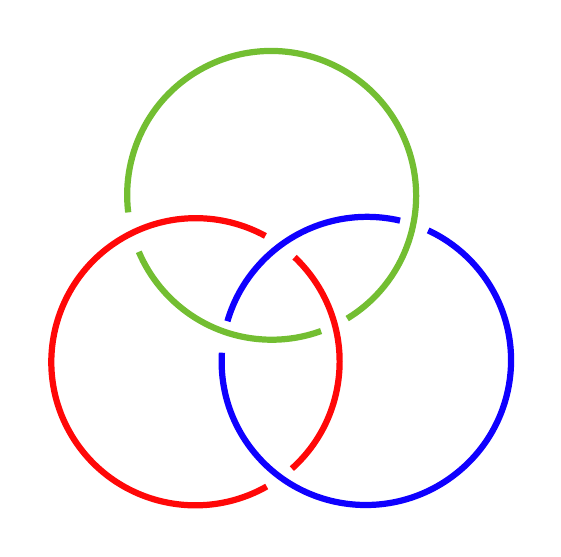
\begin{tikzpicture}[x=0.75pt,y=0.75pt,yscale=-1,xscale=1]
%uncomment if require: \path (0,300); %set diagram left start at 0, and has height of 300

%Shape: Arc [id:dp49278097545949884] 
\draw  [draw opacity=0][line width=2.25]  (328.62,163.73) .. controls (321.19,166.44) and (313.18,167.92) .. (304.82,167.92) .. controls (276.06,167.92) and (251.39,150.46) .. (240.8,125.56) -- (304.82,98.33) -- cycle ; \draw  [color={rgb, 255:red, 115; green, 190; blue, 50 }  ,draw opacity=1 ][line width=2.25]  (328.62,163.73) .. controls (321.19,166.44) and (313.18,167.92) .. (304.82,167.92) .. controls (276.06,167.92) and (251.39,150.46) .. (240.8,125.56) ;  
%Shape: Arc [id:dp7313937278600963] 
\draw  [draw opacity=0][line width=2.25]  (380.22,115.26) .. controls (389.75,119.69) and (398.4,126.36) .. (405.34,135.15) .. controls (429.07,165.23) and (423.73,208.87) .. (393.41,232.62) .. controls (363.09,256.37) and (319.27,251.24) .. (295.54,221.15) .. controls (284.6,207.29) and (279.84,190.54) .. (280.85,174.18) -- (350.44,178.15) -- cycle ; \draw  [color={rgb, 255:red, 15; green, 0; blue, 255 }  ,draw opacity=1 ][line width=2.25]  (380.22,115.26) .. controls (389.75,119.69) and (398.4,126.36) .. (405.34,135.15) .. controls (429.07,165.23) and (423.73,208.87) .. (393.41,232.62) .. controls (363.09,256.37) and (319.27,251.24) .. (295.54,221.15) .. controls (284.6,207.29) and (279.84,190.54) .. (280.85,174.18) ;  
%Shape: Arc [id:dp9082888658781946] 
\draw  [draw opacity=0][line width=2.25]  (235.71,106.58) .. controls (232.15,77.58) and (247.26,48.37) .. (275.16,35.34) .. controls (309.93,19.08) and (351.4,34.11) .. (367.78,68.91) .. controls (383.06,101.37) and (371.11,139.56) .. (341.2,157.73) -- (304.82,98.33) -- cycle ; \draw  [color={rgb, 255:red, 115; green, 190; blue, 50 }  ,draw opacity=1 ][line width=2.25]  (235.71,106.58) .. controls (232.15,77.58) and (247.26,48.37) .. (275.16,35.34) .. controls (309.93,19.08) and (351.4,34.11) .. (367.78,68.91) .. controls (383.06,101.37) and (371.11,139.56) .. (341.2,157.73) ;  
%Shape: Arc [id:dp7357603003827937] 
\draw  [draw opacity=0][line width=2.25]  (302.44,238.64) .. controls (269.08,257.52) and (226.71,245.99) .. (207.75,212.86) .. controls (188.77,179.69) and (200.44,137.44) .. (233.81,118.48) .. controls (255.62,106.09) and (281.32,106.72) .. (301.8,117.92) -- (268.17,178.53) -- cycle ; \draw  [color={rgb, 255:red, 255; green, 8; blue, 8 }  ,draw opacity=1 ][line width=2.25]  (302.44,238.64) .. controls (269.08,257.52) and (226.71,245.99) .. (207.75,212.86) .. controls (188.77,179.69) and (200.44,137.44) .. (233.81,118.48) .. controls (255.62,106.09) and (281.32,106.72) .. (301.8,117.92) ;  
%Shape: Arc [id:dp02993817280793909] 
\draw  [draw opacity=0][line width=2.25]  (283.51,159.01) .. controls (286.66,148.19) and (292.5,137.97) .. (301.03,129.39) .. controls (318.8,111.52) and (343.85,105.22) .. (366.69,110.55) -- (350.44,178.15) -- cycle ; \draw  [color={rgb, 255:red, 15; green, 0; blue, 255 }  ,draw opacity=1 ][line width=2.25]  (283.51,159.01) .. controls (286.66,148.19) and (292.5,137.97) .. (301.03,129.39) .. controls (318.8,111.52) and (343.85,105.22) .. (366.69,110.55) ;  
%Shape: Arc [id:dp6464277844327507] 
\draw  [draw opacity=0][line width=2.25]  (315.85,128.16) .. controls (331.94,143.37) and (340.46,165.99) .. (336.68,189.48) .. controls (334.06,205.76) and (325.96,219.8) .. (314.56,230.03) -- (268.17,178.53) -- cycle ; \draw  [color={rgb, 255:red, 255; green, 8; blue, 8 }  ,draw opacity=1 ][line width=2.25]  (315.85,128.16) .. controls (331.94,143.37) and (340.46,165.99) .. (336.68,189.48) .. controls (334.06,205.76) and (325.96,219.8) .. (314.56,230.03) ;  




\end{tikzpicture}
  % Make sure this file exists
			\begin{figure}
			\scalebox{0.4}{

\tikzset{every picture/.style={line width=0.75pt}} %set default line width to 0.75pt        

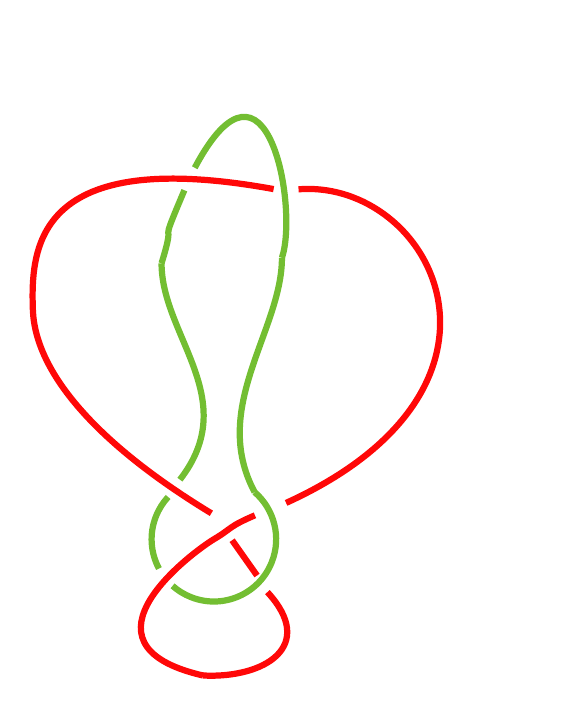
\begin{tikzpicture}[x=0.75pt,y=0.75pt,yscale=-1,xscale=1]
%uncomment if require: \path (0,300); %set diagram left start at 0, and has height of 300

%Curve Lines [id:da7443271823139895] 
\draw [color={rgb, 255:red, 255; green, 8; blue, 8 }  ,draw opacity=1 ][line width=2.25]    (343,46.68) .. controls (407,41.68) and (460,141.77) .. (337,197.77) ;
%Curve Lines [id:da24399078546827557] 
\draw [color={rgb, 255:red, 255; green, 8; blue, 8 }  ,draw opacity=1 ][line width=2.25]    (322,203.75) .. controls (309.03,209.29) and (311.19,209.93) .. (302.21,215.27) .. controls (293.23,220.61) and (231,265.75) .. (297,280.92) ;
%Curve Lines [id:da5476524533721545] 
\draw [color={rgb, 255:red, 255; green, 8; blue, 8 }  ,draw opacity=1 ][line width=2.25]    (331,46.57) .. controls (216,25.57) and (214,74.97) .. (215,104.68) .. controls (216,134.4) and (245,168.77) .. (301,202.77) ;
%Curve Lines [id:da09747722923918067] 
\draw [color={rgb, 255:red, 255; green, 8; blue, 8 }  ,draw opacity=1 ][line width=2.25]    (328,240.75) .. controls (352,266.75) and (326.73,282.41) .. (297,280.92) ;
%Shape: Arc [id:dp7905415087946832] 
\draw  [draw opacity=0][line width=2.25]  (321.85,192.58) .. controls (331.21,200.68) and (334.92,214.11) .. (330.11,226.28) .. controls (324.03,241.69) and (306.61,249.26) .. (291.19,243.17) .. controls (287.84,241.85) and (284.86,239.99) .. (282.31,237.73) -- (302.21,215.27) -- cycle ; \draw  [color={rgb, 255:red, 115; green, 190; blue, 50 }  ,draw opacity=1 ][line width=2.25]  (321.85,192.58) .. controls (331.21,200.68) and (334.92,214.11) .. (330.11,226.28) .. controls (324.03,241.69) and (306.61,249.26) .. (291.19,243.17) .. controls (287.84,241.85) and (284.86,239.99) .. (282.31,237.73) ;  
%Shape: Arc [id:dp9636288395339626] 
\draw  [draw opacity=0][line width=2.25]  (275.74,229.39) .. controls (271.75,221.9) and (270.94,212.77) .. (274.3,204.25) .. controls (275.71,200.7) and (277.71,197.56) .. (280.16,194.91) -- (302.21,215.27) -- cycle ; \draw  [color={rgb, 255:red, 115; green, 190; blue, 50 }  ,draw opacity=1 ][line width=2.25]  (275.74,229.39) .. controls (271.75,221.9) and (270.94,212.77) .. (274.3,204.25) .. controls (275.71,200.7) and (277.71,197.56) .. (280.16,194.91) ;  
%Straight Lines [id:da2186127141902522] 
\draw [color={rgb, 255:red, 255; green, 8; blue, 8 }  ,draw opacity=1 ][fill={rgb, 255:red, 208; green, 2; blue, 27 }  ,fill opacity=1 ][line width=2.25]    (311,215.75) -- (323,232.75) ;
%Curve Lines [id:da09746020631322583] 
\draw [color={rgb, 255:red, 115; green, 190; blue, 50 }  ,draw opacity=1 ][line width=2.25]    (335,79.68) .. controls (335,114.68) and (300,151.68) .. (321.85,192.58) ;
%Curve Lines [id:da25917359230011294] 
\draw [color={rgb, 255:red, 115; green, 190; blue, 50 }  ,draw opacity=1 ][line width=2.25]    (277,82.3) .. controls (277,117.3) and (316,147.68) .. (285.85,186.58) ;
%Curve Lines [id:da698321716307497] 
\draw [color={rgb, 255:red, 115; green, 190; blue, 50 }  ,draw opacity=1 ][line width=2.25]    (277,82.3) .. controls (285,56.3) and (274,80.12) .. (288,47.12) ;
%Curve Lines [id:da17510978624657203] 
\draw [color={rgb, 255:red, 115; green, 190; blue, 50 }  ,draw opacity=1 ][line width=2.25]    (335,79.68) .. controls (343,55.68) and (328,-29.7) .. (293,36.3) ;




\end{tikzpicture}
}\end{figure}
			\begin{itemize}
				\item \textbf{Eigenvalues:} {\footnotesize $\mathcolor{OliveGreen}{0.333,{\mathbf{-0.333}}, 0.666$}}
				\item \small One eigenvalue is negative $\rightarrow$ \textbf{\textcolor{OliveGreen}{Tripartite Entanglement}}
				 \end{itemize}
		\end{minipage}%
		\begin{minipage}{0.5\textwidth}
		\footnotesize
			\begin{align*}
				\rho_{ab} &=
                    \left[
                    \begin{array}{cccc}
                    0.666 & 0.0 & 0.0 & 0.333 \\
                    0.0 & 0.0 & 0.0 & 0.0 \\
                    0.0 & 0.0 & 0.0 & 0.0 \\
                    0.333 & 0.0 & 0.0 & 0.333 \\
                    \end{array}
                    \right]\\
				\mathcolor{OliveGreen}{\rho_{ab}^{T_a}} &=
                    \left[
                    \begin{array}{cccc}
                    0.666 & 0.0 & 0.0 & 0.0 \\
                    0.0 & 0.0 & 0.333 & 0.0 \\
                    0.0 & 0.333 & 0.0 & 0.0 \\
                    0.0 & 0.0 & 0.0 & 0.333 \\
                    \end{array}
                    \right]\\
				\end{align*}
		\end{minipage}
	\end{frame}




	\begin{frame}{\textbf{Three Qubit System}: 3\textsuperscript{2} class}
		\textcolor{red}{\textbf{Pure State:} } $\ket{3^2}_{abc} = \frac{1}{\sqrt{3}}\brac{\ket{000}_{abc} + \ket{111}_{abc} + \ket{001}_{abc}} $\\[0.3cm]
		\begin{minipage}{0.35\textwidth}
			%

\tikzset{every picture/.style={line width=0.75pt}} %set default line width to 0.75pt        

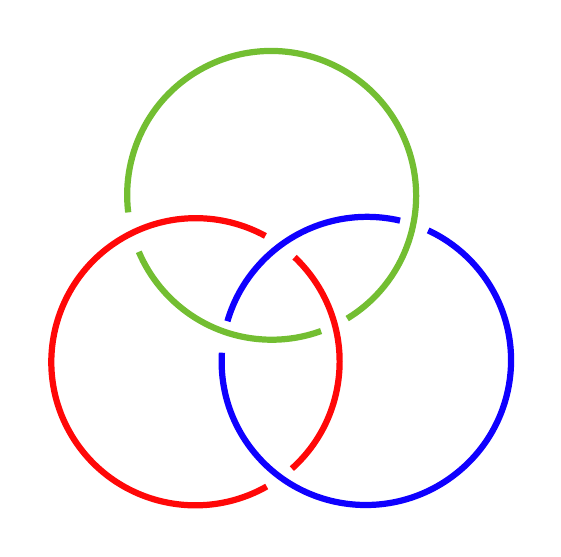
\begin{tikzpicture}[x=0.75pt,y=0.75pt,yscale=-1,xscale=1]
%uncomment if require: \path (0,300); %set diagram left start at 0, and has height of 300

%Shape: Arc [id:dp49278097545949884] 
\draw  [draw opacity=0][line width=2.25]  (328.62,163.73) .. controls (321.19,166.44) and (313.18,167.92) .. (304.82,167.92) .. controls (276.06,167.92) and (251.39,150.46) .. (240.8,125.56) -- (304.82,98.33) -- cycle ; \draw  [color={rgb, 255:red, 115; green, 190; blue, 50 }  ,draw opacity=1 ][line width=2.25]  (328.62,163.73) .. controls (321.19,166.44) and (313.18,167.92) .. (304.82,167.92) .. controls (276.06,167.92) and (251.39,150.46) .. (240.8,125.56) ;  
%Shape: Arc [id:dp7313937278600963] 
\draw  [draw opacity=0][line width=2.25]  (380.22,115.26) .. controls (389.75,119.69) and (398.4,126.36) .. (405.34,135.15) .. controls (429.07,165.23) and (423.73,208.87) .. (393.41,232.62) .. controls (363.09,256.37) and (319.27,251.24) .. (295.54,221.15) .. controls (284.6,207.29) and (279.84,190.54) .. (280.85,174.18) -- (350.44,178.15) -- cycle ; \draw  [color={rgb, 255:red, 15; green, 0; blue, 255 }  ,draw opacity=1 ][line width=2.25]  (380.22,115.26) .. controls (389.75,119.69) and (398.4,126.36) .. (405.34,135.15) .. controls (429.07,165.23) and (423.73,208.87) .. (393.41,232.62) .. controls (363.09,256.37) and (319.27,251.24) .. (295.54,221.15) .. controls (284.6,207.29) and (279.84,190.54) .. (280.85,174.18) ;  
%Shape: Arc [id:dp9082888658781946] 
\draw  [draw opacity=0][line width=2.25]  (235.71,106.58) .. controls (232.15,77.58) and (247.26,48.37) .. (275.16,35.34) .. controls (309.93,19.08) and (351.4,34.11) .. (367.78,68.91) .. controls (383.06,101.37) and (371.11,139.56) .. (341.2,157.73) -- (304.82,98.33) -- cycle ; \draw  [color={rgb, 255:red, 115; green, 190; blue, 50 }  ,draw opacity=1 ][line width=2.25]  (235.71,106.58) .. controls (232.15,77.58) and (247.26,48.37) .. (275.16,35.34) .. controls (309.93,19.08) and (351.4,34.11) .. (367.78,68.91) .. controls (383.06,101.37) and (371.11,139.56) .. (341.2,157.73) ;  
%Shape: Arc [id:dp7357603003827937] 
\draw  [draw opacity=0][line width=2.25]  (302.44,238.64) .. controls (269.08,257.52) and (226.71,245.99) .. (207.75,212.86) .. controls (188.77,179.69) and (200.44,137.44) .. (233.81,118.48) .. controls (255.62,106.09) and (281.32,106.72) .. (301.8,117.92) -- (268.17,178.53) -- cycle ; \draw  [color={rgb, 255:red, 255; green, 8; blue, 8 }  ,draw opacity=1 ][line width=2.25]  (302.44,238.64) .. controls (269.08,257.52) and (226.71,245.99) .. (207.75,212.86) .. controls (188.77,179.69) and (200.44,137.44) .. (233.81,118.48) .. controls (255.62,106.09) and (281.32,106.72) .. (301.8,117.92) ;  
%Shape: Arc [id:dp02993817280793909] 
\draw  [draw opacity=0][line width=2.25]  (283.51,159.01) .. controls (286.66,148.19) and (292.5,137.97) .. (301.03,129.39) .. controls (318.8,111.52) and (343.85,105.22) .. (366.69,110.55) -- (350.44,178.15) -- cycle ; \draw  [color={rgb, 255:red, 15; green, 0; blue, 255 }  ,draw opacity=1 ][line width=2.25]  (283.51,159.01) .. controls (286.66,148.19) and (292.5,137.97) .. (301.03,129.39) .. controls (318.8,111.52) and (343.85,105.22) .. (366.69,110.55) ;  
%Shape: Arc [id:dp6464277844327507] 
\draw  [draw opacity=0][line width=2.25]  (315.85,128.16) .. controls (331.94,143.37) and (340.46,165.99) .. (336.68,189.48) .. controls (334.06,205.76) and (325.96,219.8) .. (314.56,230.03) -- (268.17,178.53) -- cycle ; \draw  [color={rgb, 255:red, 255; green, 8; blue, 8 }  ,draw opacity=1 ][line width=2.25]  (315.85,128.16) .. controls (331.94,143.37) and (340.46,165.99) .. (336.68,189.48) .. controls (334.06,205.76) and (325.96,219.8) .. (314.56,230.03) ;  




\end{tikzpicture}
  % Make sure this file exists
			\begin{figure}
			\scalebox{0.4}{

\tikzset{every picture/.style={line width=0.75pt}} %set default line width to 0.75pt        

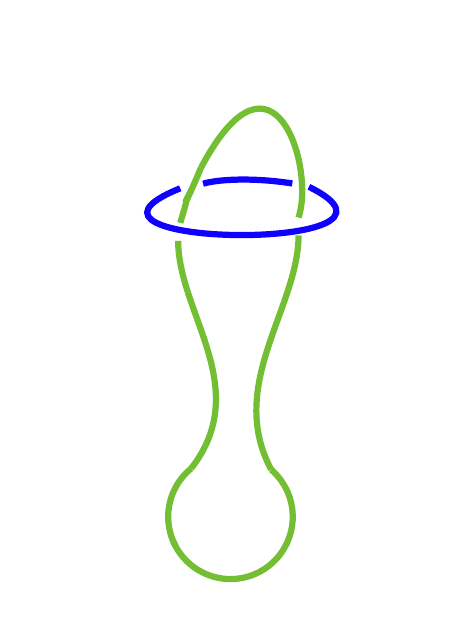
\begin{tikzpicture}[x=0.75pt,y=0.75pt,yscale=-1,xscale=1]
%uncomment if require: \path (0,300); %set diagram left start at 0, and has height of 300

%Shape: Arc [id:dp21168646143636116] 
\draw  [draw opacity=0][line width=2.25]  (321.85,192.58) .. controls (331.21,200.68) and (334.92,214.11) .. (330.11,226.28) .. controls (324.03,241.69) and (306.61,249.26) .. (291.19,243.17) .. controls (283.51,240.14) and (277.78,234.29) .. (274.71,227.27) -- (302.21,215.27) -- cycle ; \draw  [color={rgb, 255:red, 115; green, 190; blue, 50 }  ,draw opacity=1 ][line width=2.25]  (321.85,192.58) .. controls (331.21,200.68) and (334.92,214.11) .. (330.11,226.28) .. controls (324.03,241.69) and (306.61,249.26) .. (291.19,243.17) .. controls (283.51,240.14) and (277.78,234.29) .. (274.71,227.27) ;  
%Shape: Arc [id:dp7304033012343536] 
\draw  [draw opacity=0][line width=2.25]  (275.74,229.39) .. controls (271.75,221.9) and (270.94,212.77) .. (274.3,204.25) .. controls (276.26,199.3) and (279.39,195.15) .. (283.25,192.01) -- (302.21,215.27) -- cycle ; \draw  [color={rgb, 255:red, 115; green, 190; blue, 50 }  ,draw opacity=1 ][line width=2.25]  (275.74,229.39) .. controls (271.75,221.9) and (270.94,212.77) .. (274.3,204.25) .. controls (276.26,199.3) and (279.39,195.15) .. (283.25,192.01) ;  
%Curve Lines [id:da08845374014848362] 
\draw [color={rgb, 255:red, 115; green, 190; blue, 50 }  ,draw opacity=1 ][line width=2.25]    (335,79.68) .. controls (335,114.68) and (300,151.68) .. (321.85,192.58) ;
%Curve Lines [id:da38795962135966966] 
\draw [color={rgb, 255:red, 115; green, 190; blue, 50 }  ,draw opacity=1 ][line width=2.25]    (277,82.3) .. controls (277,117.3) and (313.4,153.11) .. (283.25,192.01) ;
%Curve Lines [id:da55034677237778] 
\draw [color={rgb, 255:red, 115; green, 190; blue, 50 }  ,draw opacity=1 ][line width=2.25]    (278,73.65) .. controls (286,47.65) and (274,80.12) .. (288,47.12) ;
%Curve Lines [id:da8611153062481857] 
\draw [color={rgb, 255:red, 115; green, 190; blue, 50 }  ,draw opacity=1 ][line width=2.25]    (335,71.12) .. controls (343,47.12) and (323,-18.88) .. (288,47.12) ;
%Curve Lines [id:da7227634588793097] 
\draw [color={rgb, 255:red, 15; green, 0; blue, 255 }  ,draw opacity=1 ][line width=2.25]    (278,57.02) .. controls (206,86.02) and (405,88.3) .. (340,56.3) ;
%Curve Lines [id:da6158714712059778] 
\draw [color={rgb, 255:red, 15; green, 0; blue, 255 }  ,draw opacity=1 ][line width=2.25]    (289,54.8) .. controls (296,52.68) and (313,51.68) .. (332,54.68) ;




\end{tikzpicture}
}\end{figure}
			\begin{itemize}
				\item \textbf{Eigenvalues:} {\footnotesize{\footnotesize $\mathcolor{red}{ 0.0, 0.333, 0.666$}}}
				\item \small No eigenvalue is negative $\rightarrow$ \textbf{\textcolor{red}{Separable}}
				 \end{itemize}
		\end{minipage}%
		\begin{minipage}{0.5\textwidth}
		\footnotesize
			\begin{align*}
					\rho_{bc} &=
					\left[
					\begin{array}{cccc}
					0.333 & 0.333 & 0.0 & 0.0 \\
					0.333 & 0.333 & 0.0 & 0.0 \\
					0.0 & 0.0 & 0.0 & 0.0 \\
					0.0 & 0.0 & 0.0 & 0.333 \\
					\end{array}
					\right]\\
					\mathcolor{red}{\rho^{T_b}_{bc}}&=
                \left[
                \begin{array}{cccc}
                0.333 & 0.333 & 0.0 & 0.0 \\
                0.333 & 0.333 & 0.0 & 0.0 \\
                0.0 & 0.0 & 0.0 & 0.0 \\
                0.0 & 0.0 & 0.0 & 0.333 \\
                \end{array}
                \right]
				\end{align*}
		\end{minipage}
	\end{frame}





	\begin{frame}{\textbf{Three Qubit System}: 3\textsuperscript{3} class}
		
	\end{frame}
	\begin{frame}{\textbf{Three Qubit System}: 3\textsuperscript{4} class}
		
	\end{frame}
	\begin{frame}{\textbf{Four Qubit System}}
		
	\end{frame}
	\begin{frame}{\textbf{Application to Qubit Networks}}
		
	\end{frame}
	
	\begin{frame}{\textbf{Conclusion}}
		
	\end{frame}
\end{document}